\section{Topology coverage control}

Motivation: Roles need to be assigned to nodes. Nodes which aren't needed
should sleep.

\begin{description}
		\item[Topology coverage] Govern which nodes are required to provide
				communication network. Dependant on tx/rx capabilities.
		\item[Coverage control] Governs which nodes are required to cover
				desired area. Dependant on sensing capabilities.
\end{description}


\subsection{Topology coverage}

\begin{itemize}
		\item Must be energy-efficient, scalable, distributed, robust. Topology
				consists of set of active nodes $V$ and set of active links
				$E$.
		\item Topology control transform $(V, E)$ to $(V', E')$ by switching
				off (or back on) nodes in $V$, and limiting transmission power
				which will adjust $E$.
		\item Active links can be arranged hierarchical. Set of backbone nodes
				forming a ``connected dominating set'' (CDS). All non-backbone
				nodes connect only to backbone nodes. Backbone nodes may
				connect to anyone.
		\item Experiments show that, as transmission range increased, there's a
				certain point where connectivity (in percentage of total nodes
				reachable) rises sharply.  Ideally just above that point.
		\item Routing and topology control interact. E.g. if packet not
				deliverable, topology control must act.
\end{itemize}

\subsubsection{Flat topology control protocols}

\paragraph{Relative Neighborhood Graph, RNG}

RNG $T = (V, E')$ of graph $G = (V, E)$ is defined as:
\begin{align*}
		\forall u, v \in V: (u, v) \in E' \Leftrightarrow \not\exists w \in V: max(d(u, w), d(v, w)) < d(u, v)
\end{align*}

In words: Two nodes are connected IFF there is no other node that, if they were
connected via it, the longer of the two new connections would be shorter than
the existing one. Example: Edge between the blue ones not in RNG as each of the
blue-red edges would be shorter than the blue-blue one.

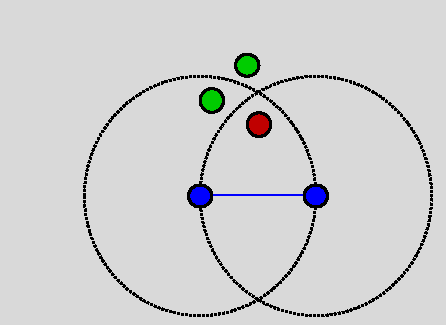
\includegraphics[width=0.5\textwidth]{06_rng}

\paragraph{Gabriel Graph, GG}

GG $T = (V, E')$ of $G = (V, E)$ is defined as:
\begin{align*}
		\forall u, v \in V: (u, v) \in E' \Leftrightarrow \not \exists w \in V : d^2(u, w) + d^2(v, w) < d^2(u, v)
\end{align*}

RNG is subgraph of GG.

\paragraph{Delaunay triangulation, DT}

The DT of a set of $n$ points $P$ is the unique triangulation such that the
cirumcircle of every triangle contains no points of $P$ in its interior.

\paragraph{Local Minimum Spanning Tree}

\begin{itemize}
		\item Beacons exchange information with max tx power, learn who their 1-hop neighbours are
		\item Construction of local minimum spanning tree \textbf{containing all 1-hop neighbours}
				\begin{itemize}
						\item Connections not necessarily the direct path! Can go via other neighbour.
				\end{itemize}
		\item Node $v$ is kept in neighbor list of node IFF it is a 1-hop
				neighbour \textbf{in its minimum spanning tree}
\end{itemize}

Example: Red is 1-hop neighbour of blue, but not 1-hop neighbour in its minimum
spanning tree, as cheaper connection via green (top right).

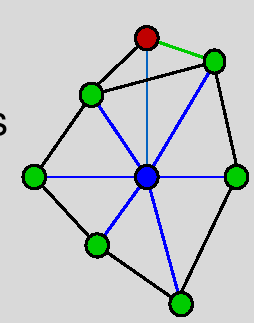
\includegraphics[width=0.5\textwidth]{06_lmst}

\paragraph{Cone-based topology control}

\begin{itemize}
		\item Each node splits its radial area into $n$ cones of angle $\alpha$
				(such that $n \cdot \alpha = 360$).
		\item Then, starting with a low TX power it sends beacons.
		\item Increases TX power until there's at least one neighbour in each cone.
		\item If there are two edges $(u, v_1)$, $(u, v_2)$, the longer can be
				removed if $d(v_1, v_2) < max(d(u, v_1), d(u, v_2))$
\end{itemize}


\paragraph{COMPOW}

\begin{itemize}
		\item Assume node has power levels
		\item Node selects lowest power level having same number of reachable
				nodes as maximum power level
		\item Enabled by one routing protocol per power level. But causes
				overheads, as multiple routing layers active.
\end{itemize}

\subsubsection{Hierarchical topology control}

Idea: Select virtual backbone of nodes which remain active.

\paragraph{Minimum connected dominating sets, MCDS}

Dominating set is subset $D$ of $V$ where each node in $V \setminus D$ is
adjacent to some node in $D$. That is every node eitehr is in D, or has an edge
connecting it to a node in D.

Connected dominating set is a dominating set which builds a connected sub-graph
of the network.

Minimum cds is the CDS containing the least amount of nodes. Finding it is
NP-complete, but heuristics exists, such as MPR-CDS.

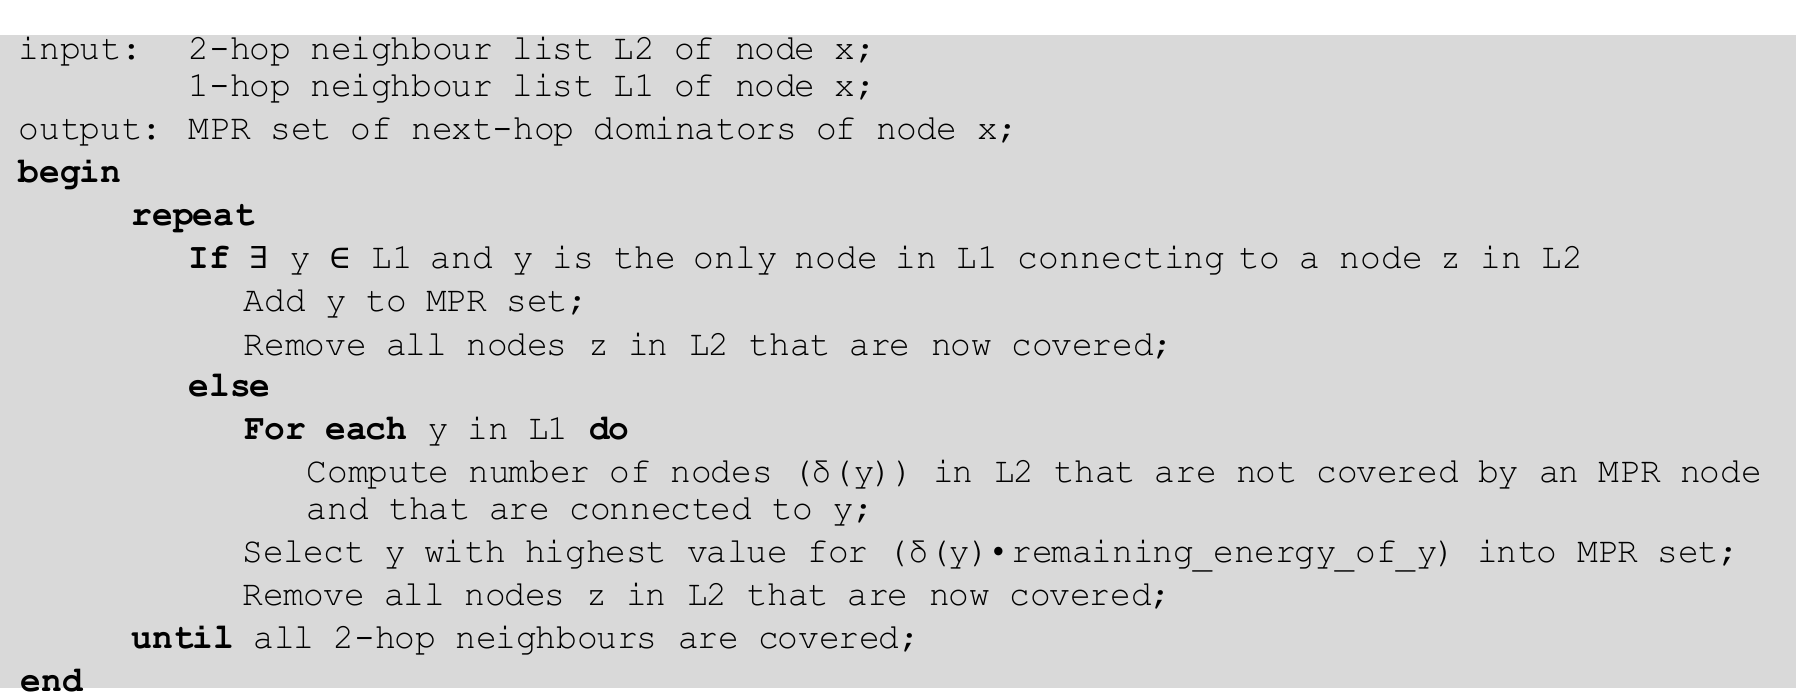
\includegraphics[width=\textwidth]{06_mpr_cds}

\paragraph{SPAN}

\begin{itemize}
		\item Node periodically announces willingness to become coordinator
				(part of backbone) if it discovers that two neighbours cannot
				communicate via at most 2 backbone nodes.
		\item When node wants to withdraw as coordinator it announces itself as
				tentative. If none objects, it withdraws.
		\item Randomized back-off delay for announcements.
\end{itemize}

\paragraph{Geographic adapative fidelity}

\begin{itemize}
		\item Nodes on virtual grid, can communicate if in adjacent cells
		\item One node per cell chosen to always be active
		\item Active node sleeps if more suitable node detected, based on e.g.
				node lifetime.
\end{itemize}

\subsection{Coverage control}

\subsubsection{Probeing Environment and Adaptive Sleeping, PEAS}

\begin{itemize}
		\item Sensor nodes sleep, wake up periodically, send probing message
		\item Receiving sensors estimate distance to probing sensor. If too
				close they announce their presence, probing node sleeps again.
		\item Otherwise, probing node becomes active
		\item Probing frequency balances energy usage and robustness
\end{itemize}

\subsubsection{Node-self-scheduling scheme, NSSS}

\begin{itemize}
		\item Node measures neighbourhood redundancy as union of sectors covered by neighbouring sensors
		\item If full \SI{360}{\degree} covered, node can withdraw
		\item Problem: Node failures
\end{itemize}

\subsubsection{Gur Game}

\begin{itemize}
		\item Sensors run FSM split in two halves. Left: No data sent. Right: Data sent.
		\item Base station calculates and broadcasts $r = f(\text{received
				packets})$, which is function which max at desired number of
				packets.
		\item Nodes move, with probability $r$, towards the edge, with $1 - r$
				towards the center of the FSM.
\end{itemize}

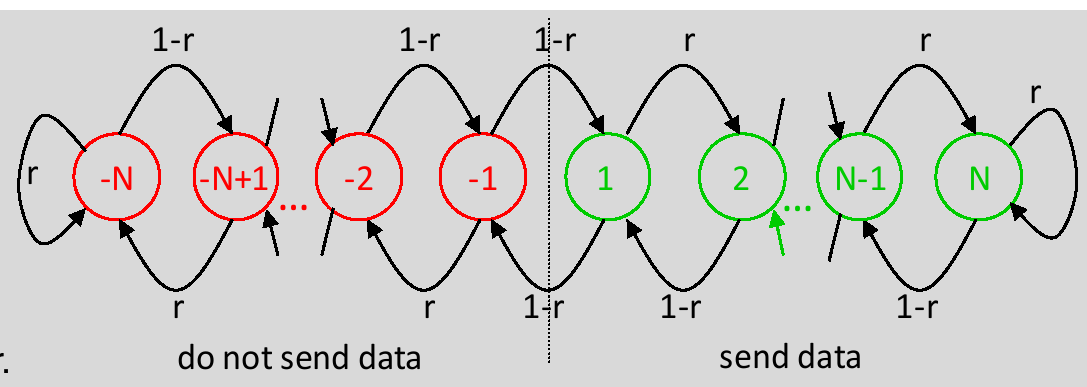
\includegraphics[width=\textwidth]{06_gur_game}

\subsubsection{Reference time-based scheduling scheme}

\begin{itemize}
		\item Divide environment into grid. Assume tx radius > 2 sensing radius
		\item Broadcast randomly chosen reference time in $[0, T)$, $T$ round length
		\item For each grid point, sensor sorts reference time of sensors able to monitor (= reach) it
		\item Schedules its own activity centered on its own reference time,
				such that it reaches at most halfway towards the next lower and
				higher reference times.
\end{itemize}

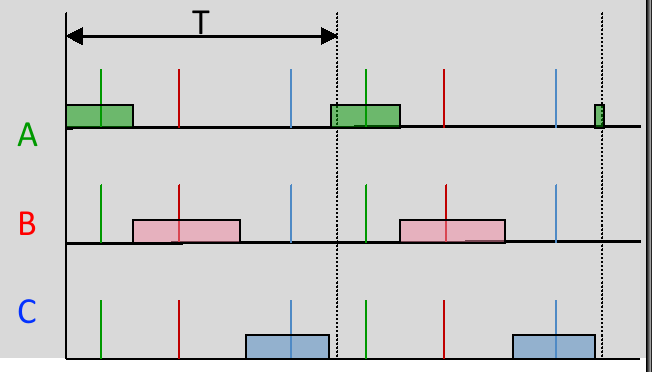
\includegraphics[width=\textwidth]{06_reference_time}

\subsubsection{Coverage configuration protocol, CCP}

\begin{itemize}
		\item Node determines intersection points between coverage area and neighbours' sensing radii
		\item Node sleeps if each intersection point covered by at least $k$ neighbours
\end{itemize}

\subsection{Combining topology and coverage control}

Problem: Topology control has no knowledge of traffic patterns. Often traffic
from select few nodes, and topology control maintains too big a communication
network.

\subsubsection{Connected sensor cover}

Idea: Find minimum number of nodes to cover area.

\begin{itemize}
		\item If $M$ set of covered sensors
		\item Find candidates with sensing region intersecting that of M
		\item Find path $P_i$ to every candidate (starting in M) with highest
				benefit (additional coverage for $M$)
		\item Add path with highest benefit, add candidates along that path
\end{itemize}

\subsubsection{Distributed activation with pre-determined routes}

Idea: Important or low-energy nodes should not be used for sensing.

\begin{itemize}
		\item Each node assigns itself a cost
		\item Route discovery using cost as routing metric
		\item Nodes activate themselves after back-off delay proportional to activation cost. No activation if neighbourhood covered
		\item Nodes deactivate themselves if they discover redundant nodes.
\end{itemize}
